%%%% Paramétrage du TD %%%%
\def\xxactivite{ \ifprof \normalsize{Activation 1 -- Corrigé } \else  \ifcolle Colle \else Activation 1\fi \fi} % \normalsize \vspace{-.4cm}
\def\xxauteur{\textsl{Xavier Pessoles}}


\def\xxnumchapitre{Chapitre 2 \vspace{.2cm}}
\def\xxchapitre{\hspace{.12cm} Hyperstatisme}



\def\xxcompetences{%
\textsl{%
\textbf{Savoirs et compétences :}\\
\begin{itemize}[label=\ding{112},font=\color{ocre}] 
\item \textit{Mod2.C34} : chaînes de solides.
%\item \textit{Mod2.C34} : degré de mobilité du modèle;
%\item \textit{Mod2.C34} : degré d’hyperstatisme du modèle;
%\item \textit{Mod2.C34.SF1} : déterminer les conditions géométriques associées à l’hyperstatisme;
%\item \textit{Mod2.C34} : résoudre le système associé à la fermeture cinématique et en déduire le degré de mobilité et d’hyperstatisme.
\end{itemize}
}}

\def\xxtitreexo{Activation -- Pompe à pistons axiaux}
\def\xxsourceexo{\hspace{.2cm} \footnotesize{\'E. Durif}}


\def\xxfigures{
%\includegraphics[width=.7\linewidth]{axe_y_photo}
}%figues de la page de garde


\iflivret
\pagestyle{empty}


%%%%%%%% PAGE DE GARDE COURS
\ifcours
% ==== BANDEAU DES TITRES ==== 
\begin{tikzpicture}[remember picture,overlay]
\node at (current page.north west)
{\begin{tikzpicture}[remember picture,overlay]
\node[anchor=north west,inner sep=0pt] at (0,0) {\includegraphics[width=\paperwidth]{\thechapterimage}};
\draw[anchor=west] (-2cm,-8cm) node [line width=2pt,rounded corners=15pt,draw=ocre,fill=white,fill opacity=0.6,inner sep=40pt]{\strut\makebox[22cm]{}};
\draw[anchor=west] (1cm,-8cm) node {\huge\sffamily\bfseries\color{black} %
\begin{minipage}{1cm}
\rotatebox{90}{\LARGE\sffamily\textsc{\color{ocre}\textbf{\xxnumpartie}}}
\end{minipage} \hfill
\begin{minipage}[c]{14cm}
\begin{titrepartie}
\begin{flushright}
\renewcommand{\baselinestretch}{1.1} 
\Large\sffamily\textsc{\textbf{\xxpartie}}
\renewcommand{\baselinestretch}{1} 
\end{flushright}
\end{titrepartie}
\end{minipage} \hfill
\begin{minipage}[c]{3.5cm}
{\large\sffamily\textsc{\textbf{\color{ocre} \discipline}}}
\end{minipage} 
 };
\end{tikzpicture}};
\end{tikzpicture}
% ==== FIN BANDEAU DES TITRES ==== 


% ==== ONGLET 
\begin{tikzpicture}[overlay]
\node[shape=rectangle, 
      rounded corners = .25 cm,
	  draw= ocre,
	  line width=2pt, 
	  fill = ocre!10,
	  minimum width  = 2.5cm,
	  minimum height = 3cm,] at (18.3cm,0) {};
\node at (17.7cm,0) {\rotatebox{90}{\textbf{\Large\color{ocre}{\classe}}}};
%{};
\end{tikzpicture}
% ==== FIN ONGLET 


\vspace{3.5cm}

\begin{tikzpicture}[remember picture,overlay]
\draw[anchor=west] (-2cm,-6cm) node {\huge\sffamily\bfseries\color{black} %
\begin{minipage}{2cm}
\begin{center}
\LARGE\sffamily\textsc{\color{ocre}\textbf{\xxactivite}}
\end{center}
\end{minipage} \hfill
\begin{minipage}[c]{15cm}
\begin{titrechapitre}
\renewcommand{\baselinestretch}{1.1} 
\Large\sffamily\textsc{\textbf{\xxnumchapitre}}

\Large\sffamily\textsc{\textbf{\xxchapitre}}
\vspace{.5cm}

\renewcommand{\baselinestretch}{1} 
\normalsize\normalfont
\xxcompetences
\end{titrechapitre}
\end{minipage}  };
\end{tikzpicture}
\vfill

\begin{flushright}
\begin{minipage}[c]{.3\linewidth}
\begin{center}
\xxfigures
\end{center}
\end{minipage}\hfill
\begin{minipage}[c]{.6\linewidth}
\startcontents
%\printcontents{}{1}{}
\printcontents{}{1}{}
\end{minipage}
\end{flushright}

\begin{tikzpicture}[remember picture,overlay]
\draw[anchor=west] (4.5cm,-.7cm) node {
\begin{minipage}[c]{.2\linewidth}
\begin{flushright}

\includegraphics[width=2cm]{logoCC}
\end{flushright}
\end{minipage}
\begin{minipage}[c]{.2\linewidth}
\textsl{\xxauteur} \\
\textsl{\classe}
\end{minipage}
 };
\end{tikzpicture}

\newpage
\pagestyle{fancy}

%\newpage
%\pagestyle{fancy}

\else
\fi
%% FIN PAGE DE GARDE DES COURS

%%%%%%%% PAGE DE GARDE TD
\iftd
%\begin{tikzpicture}[remember picture,overlay]
%\node at (current page.north west)
%{\begin{tikzpicture}[remember picture,overlay]
%\draw[anchor=west] (-2cm,-3.25cm) node [line width=2pt,rounded corners=15pt,draw=ocre,fill=white,fill opacity=0.6,inner sep=40pt]{\strut\makebox[22cm]{}};
%\draw[anchor=west] (1cm,-3.25cm) node {\huge\sffamily\bfseries\color{black} %
%\begin{minipage}{1cm}
%\rotatebox{90}{\LARGE\sffamily\textsc{\color{ocre}\textbf{\xxnumpartie}}}
%\end{minipage} \hfill
%\begin{minipage}[c]{13.5cm}
%\begin{titrepartie}
%\begin{flushright}
%\renewcommand{\baselinestretch}{1.1} 
%\Large\sffamily\textsc{\textbf{\xxpartie}}
%\renewcommand{\baselinestretch}{1} 
%\end{flushright}
%\end{titrepartie}
%\end{minipage} \hfill
%\begin{minipage}[c]{3.5cm}
%{\large\sffamily\textsc{\textbf{\color{ocre} \discipline}}}
%\end{minipage} 
% };
%\end{tikzpicture}};
%\end{tikzpicture}

%%%%%%%%%% PAGE DE GARDE TD %%%%%%%%%%%%%%%
%\begin{tikzpicture}[overlay]
%\node[shape=rectangle, 
%      rounded corners = .25 cm,
%	  draw= ocre,
%	  line width=2pt, 
%	  fill = ocre!10,
%	  minimum width  = 2.5cm,
%	  minimum height = 2.5cm,] at (18.5cm,0) {};
%\node at (17.7cm,0) {\rotatebox{90}{\textbf{\Large\color{ocre}{\classe}}}};
%%{};
%\end{tikzpicture}

% PARTIE ET CHAPITRE
%\begin{tikzpicture}[remember picture,overlay]
%\draw[anchor=west] (-1cm,-2.1cm) node {\large\sffamily\bfseries\color{black} %
%\begin{minipage}[c]{15cm}
%\begin{flushleft}
%\xxnumchapitre \\
%\xxchapitre
%\end{flushleft}
%\end{minipage}  };
%\end{tikzpicture}

% BANDEAU EXO
\iflivret % SI LIVRET
\begin{tikzpicture}[remember picture,overlay]
\draw[anchor=west] (-2cm,-3.3cm) node {\huge\sffamily\bfseries\color{black} %
\begin{minipage}{5cm}
\begin{center}
\LARGE\sffamily\color{ocre}\textbf{\textsc{\xxactivite}}

\begin{center}
\xxfigures
\end{center}

\end{center}
\end{minipage} \hfill
\begin{minipage}[c]{12cm}
\begin{titrechapitre}
\renewcommand{\baselinestretch}{1.1} 
\large\sffamily\textbf{\textsc{\xxtitreexo}}

\small\sffamily{\textbf{\textit{\color{black!70}\xxsourceexo}}}
\vspace{.5cm}

\renewcommand{\baselinestretch}{1} 
\normalsize\normalfont
\xxcompetences
\end{titrechapitre}
\end{minipage}};
\end{tikzpicture}
\else % ELSE NOT LIVRET
\begin{tikzpicture}[remember picture,overlay]
\draw[anchor=west] (-2cm,-4.5cm) node {\huge\sffamily\bfseries\color{black} %
\begin{minipage}{5cm}
\begin{center}
\LARGE\sffamily\color{ocre}\textbf{\textsc{\xxactivite}}

\begin{center}
\xxfigures
\end{center}

\end{center}
\end{minipage} \hfill
\begin{minipage}[c]{12cm}
\begin{titrechapitre}
\renewcommand{\baselinestretch}{1.1} 
\large\sffamily\textbf{\textsc{\xxtitreexo}}

\small\sffamily{\textbf{\textit{\color{black!70}\xxsourceexo}}}
\vspace{.5cm}

\renewcommand{\baselinestretch}{1} 
\normalsize\normalfont
\xxcompetences
\end{titrechapitre}
\end{minipage}};
\end{tikzpicture}

\fi

\else   % FIN IF TD
\fi


%%%%%%%% PAGE DE GARDE FICHE
\iffiche
\begin{tikzpicture}[remember picture,overlay]
\node at (current page.north west)
{\begin{tikzpicture}[remember picture,overlay]
\draw[anchor=west] (-2cm,-2.25cm) node [line width=2pt,rounded corners=15pt,draw=ocre,fill=white,fill opacity=0.6,inner sep=40pt]{\strut\makebox[22cm]{}};
\draw[anchor=west] (1cm,-2.25cm) node {\huge\sffamily\bfseries\color{black} %
\begin{minipage}{1cm}
\rotatebox{90}{\LARGE\sffamily\textsc{\color{ocre}\textbf{\xxnumpartie}}}
\end{minipage} \hfill
\begin{minipage}[c]{14cm}
\begin{titrepartie}
\begin{flushright}
\renewcommand{\baselinestretch}{1.1} 
\large\sffamily\textsc{\textbf{\xxpartie} \\} 

\vspace{.2cm}

\normalsize\sffamily\textsc{\textbf{\xxnumchapitre -- \xxchapitre}}
\renewcommand{\baselinestretch}{1} 
\end{flushright}
\end{titrepartie}
\end{minipage} \hfill
\begin{minipage}[c]{3.5cm}
{\large\sffamily\textsc{\textbf{\color{ocre} \discipline}}}
\end{minipage} 
 };
\end{tikzpicture}};
\end{tikzpicture}

\iflivret
\begin{tikzpicture}[overlay]
\node[shape=rectangle, 
      rounded corners = .25 cm,
	  draw= ocre,
	  line width=2pt, 
	  fill = ocre!10,
	  minimum width  = 2.5cm,
	  minimum height = 2.5cm,] at (18.5cm,1.1cm) {};
\node at (17.9cm,1.1cm) {\rotatebox{90}{\textsf{\textbf{\large\color{ocre}{\classe}}}}};
%{};
\end{tikzpicture}
\else
\begin{tikzpicture}[overlay]
\node[shape=rectangle, 
      rounded corners = .25 cm,
	  draw= ocre,
	  line width=2pt, 
	  fill = ocre!10,
	  minimum width  = 2.5cm,
%	  minimum height = 2.5cm,] at (18.5cm,1.1cm) {};
	  minimum height = 2.5cm,] at (18.6cm,0cm) {};
\node at (18cm,0cm) {\rotatebox{90}{\textsf{\textbf{\large\color{ocre}{\classe}}}}};
%{};
\end{tikzpicture}

\fi

\else
\fi



\else
\pagestyle{empty}


%%%%%%%% PAGE DE GARDE COURS
\ifcours
% ==== BANDEAU DES TITRES ==== 
\begin{tikzpicture}[remember picture,overlay]
\node at (current page.north west)
{\begin{tikzpicture}[remember picture,overlay]
\node[anchor=north west,inner sep=0pt] at (0,0) {\includegraphics[width=\paperwidth]{\thechapterimage}};
\draw[anchor=west] (-2cm,-8cm) node [line width=2pt,rounded corners=15pt,draw=ocre,fill=white,fill opacity=0.6,inner sep=40pt]{\strut\makebox[22cm]{}};
\draw[anchor=west] (1cm,-8cm) node {\huge\sffamily\bfseries\color{black} %
\begin{minipage}{1cm}
\rotatebox{90}{\LARGE\sffamily\textsc{\color{ocre}\textbf{\xxnumpartie}}}
\end{minipage} \hfill
\begin{minipage}[c]{14cm}
\begin{titrepartie}
\begin{flushright}
\renewcommand{\baselinestretch}{1.1} 
\Large\sffamily\textsc{\textbf{\xxpartie}}
\renewcommand{\baselinestretch}{1} 
\end{flushright}
\end{titrepartie}
\end{minipage} \hfill
\begin{minipage}[c]{3.5cm}
{\large\sffamily\textsc{\textbf{\color{ocre} \discipline}}}
\end{minipage} 
 };
\end{tikzpicture}};
\end{tikzpicture}
% ==== FIN BANDEAU DES TITRES ==== 


% ==== ONGLET 
\begin{tikzpicture}[overlay]
\node[shape=rectangle, 
      rounded corners = .25 cm,
	  draw= ocre,
	  line width=2pt, 
	  fill = ocre!10,
	  minimum width  = 2.5cm,
	  minimum height = 3cm,] at (18.3cm,0) {};
\node at (17.7cm,0) {\rotatebox{90}{\textbf{\Large\color{ocre}{\classe}}}};
%{};
\end{tikzpicture}
% ==== FIN ONGLET 


\vspace{3.5cm}

\begin{tikzpicture}[remember picture,overlay]
\draw[anchor=west] (-2cm,-6cm) node {\huge\sffamily\bfseries\color{black} %
\begin{minipage}{2cm}
\begin{center}
\LARGE\sffamily\textsc{\color{ocre}\textbf{\xxactivite}}
\end{center}
\end{minipage} \hfill
\begin{minipage}[c]{15cm}
\begin{titrechapitre}
\renewcommand{\baselinestretch}{1.1} 
\Large\sffamily\textsc{\textbf{\xxnumchapitre}}

\Large\sffamily\textsc{\textbf{\xxchapitre}}
\vspace{.5cm}

\renewcommand{\baselinestretch}{1} 
\normalsize\normalfont
\xxcompetences
\end{titrechapitre}
\end{minipage}  };
\end{tikzpicture}
\vfill

\begin{flushright}
\begin{minipage}[c]{.3\linewidth}
\begin{center}
\xxfigures
\end{center}
\end{minipage}\hfill
\begin{minipage}[c]{.6\linewidth}
\startcontents
%\printcontents{}{1}{}
\printcontents{}{1}{}
\end{minipage}
\end{flushright}

\begin{tikzpicture}[remember picture,overlay]
\draw[anchor=west] (4.5cm,-.7cm) node {
\begin{minipage}[c]{.2\linewidth}
\begin{flushright}

\includegraphics[width=2cm]{logoCC}
\end{flushright}
\end{minipage}
\begin{minipage}[c]{.2\linewidth}
\textsl{\xxauteur} \\
\textsl{\classe}
\end{minipage}
 };
\end{tikzpicture}

\newpage
\pagestyle{fancy}

%\newpage
%\pagestyle{fancy}

\else
\fi
%% FIN PAGE DE GARDE DES COURS

%%%%%%%% PAGE DE GARDE TD
\iftd
%\begin{tikzpicture}[remember picture,overlay]
%\node at (current page.north west)
%{\begin{tikzpicture}[remember picture,overlay]
%\draw[anchor=west] (-2cm,-3.25cm) node [line width=2pt,rounded corners=15pt,draw=ocre,fill=white,fill opacity=0.6,inner sep=40pt]{\strut\makebox[22cm]{}};
%\draw[anchor=west] (1cm,-3.25cm) node {\huge\sffamily\bfseries\color{black} %
%\begin{minipage}{1cm}
%\rotatebox{90}{\LARGE\sffamily\textsc{\color{ocre}\textbf{\xxnumpartie}}}
%\end{minipage} \hfill
%\begin{minipage}[c]{13.5cm}
%\begin{titrepartie}
%\begin{flushright}
%\renewcommand{\baselinestretch}{1.1} 
%\Large\sffamily\textsc{\textbf{\xxpartie}}
%\renewcommand{\baselinestretch}{1} 
%\end{flushright}
%\end{titrepartie}
%\end{minipage} \hfill
%\begin{minipage}[c]{3.5cm}
%{\large\sffamily\textsc{\textbf{\color{ocre} \discipline}}}
%\end{minipage} 
% };
%\end{tikzpicture}};
%\end{tikzpicture}

%%%%%%%%%% PAGE DE GARDE TD %%%%%%%%%%%%%%%
%\begin{tikzpicture}[overlay]
%\node[shape=rectangle, 
%      rounded corners = .25 cm,
%	  draw= ocre,
%	  line width=2pt, 
%	  fill = ocre!10,
%	  minimum width  = 2.5cm,
%	  minimum height = 2.5cm,] at (18.5cm,0) {};
%\node at (17.7cm,0) {\rotatebox{90}{\textbf{\Large\color{ocre}{\classe}}}};
%%{};
%\end{tikzpicture}

% PARTIE ET CHAPITRE
%\begin{tikzpicture}[remember picture,overlay]
%\draw[anchor=west] (-1cm,-2.1cm) node {\large\sffamily\bfseries\color{black} %
%\begin{minipage}[c]{15cm}
%\begin{flushleft}
%\xxnumchapitre \\
%\xxchapitre
%\end{flushleft}
%\end{minipage}  };
%\end{tikzpicture}

% BANDEAU EXO
\iflivret % SI LIVRET
\begin{tikzpicture}[remember picture,overlay]
\draw[anchor=west] (-2cm,-3.3cm) node {\huge\sffamily\bfseries\color{black} %
\begin{minipage}{5cm}
\begin{center}
\LARGE\sffamily\color{ocre}\textbf{\textsc{\xxactivite}}

\begin{center}
\xxfigures
\end{center}

\end{center}
\end{minipage} \hfill
\begin{minipage}[c]{12cm}
\begin{titrechapitre}
\renewcommand{\baselinestretch}{1.1} 
\large\sffamily\textbf{\textsc{\xxtitreexo}}

\small\sffamily{\textbf{\textit{\color{black!70}\xxsourceexo}}}
\vspace{.5cm}

\renewcommand{\baselinestretch}{1} 
\normalsize\normalfont
\xxcompetences
\end{titrechapitre}
\end{minipage}};
\end{tikzpicture}
\else % ELSE NOT LIVRET
\begin{tikzpicture}[remember picture,overlay]
\draw[anchor=west] (-2cm,-4.5cm) node {\huge\sffamily\bfseries\color{black} %
\begin{minipage}{5cm}
\begin{center}
\LARGE\sffamily\color{ocre}\textbf{\textsc{\xxactivite}}

\begin{center}
\xxfigures
\end{center}

\end{center}
\end{minipage} \hfill
\begin{minipage}[c]{12cm}
\begin{titrechapitre}
\renewcommand{\baselinestretch}{1.1} 
\large\sffamily\textbf{\textsc{\xxtitreexo}}

\small\sffamily{\textbf{\textit{\color{black!70}\xxsourceexo}}}
\vspace{.5cm}

\renewcommand{\baselinestretch}{1} 
\normalsize\normalfont
\xxcompetences
\end{titrechapitre}
\end{minipage}};
\end{tikzpicture}

\fi

\else   % FIN IF TD
\fi


%%%%%%%% PAGE DE GARDE FICHE
\iffiche
\begin{tikzpicture}[remember picture,overlay]
\node at (current page.north west)
{\begin{tikzpicture}[remember picture,overlay]
\draw[anchor=west] (-2cm,-2.25cm) node [line width=2pt,rounded corners=15pt,draw=ocre,fill=white,fill opacity=0.6,inner sep=40pt]{\strut\makebox[22cm]{}};
\draw[anchor=west] (1cm,-2.25cm) node {\huge\sffamily\bfseries\color{black} %
\begin{minipage}{1cm}
\rotatebox{90}{\LARGE\sffamily\textsc{\color{ocre}\textbf{\xxnumpartie}}}
\end{minipage} \hfill
\begin{minipage}[c]{14cm}
\begin{titrepartie}
\begin{flushright}
\renewcommand{\baselinestretch}{1.1} 
\large\sffamily\textsc{\textbf{\xxpartie} \\} 

\vspace{.2cm}

\normalsize\sffamily\textsc{\textbf{\xxnumchapitre -- \xxchapitre}}
\renewcommand{\baselinestretch}{1} 
\end{flushright}
\end{titrepartie}
\end{minipage} \hfill
\begin{minipage}[c]{3.5cm}
{\large\sffamily\textsc{\textbf{\color{ocre} \discipline}}}
\end{minipage} 
 };
\end{tikzpicture}};
\end{tikzpicture}

\iflivret
\begin{tikzpicture}[overlay]
\node[shape=rectangle, 
      rounded corners = .25 cm,
	  draw= ocre,
	  line width=2pt, 
	  fill = ocre!10,
	  minimum width  = 2.5cm,
	  minimum height = 2.5cm,] at (18.5cm,1.1cm) {};
\node at (17.9cm,1.1cm) {\rotatebox{90}{\textsf{\textbf{\large\color{ocre}{\classe}}}}};
%{};
\end{tikzpicture}
\else
\begin{tikzpicture}[overlay]
\node[shape=rectangle, 
      rounded corners = .25 cm,
	  draw= ocre,
	  line width=2pt, 
	  fill = ocre!10,
	  minimum width  = 2.5cm,
%	  minimum height = 2.5cm,] at (18.5cm,1.1cm) {};
	  minimum height = 2.5cm,] at (18.6cm,0cm) {};
\node at (18cm,0cm) {\rotatebox{90}{\textsf{\textbf{\large\color{ocre}{\classe}}}}};
%{};
\end{tikzpicture}

\fi

\else
\fi



\fi
\setlength{\columnseprule}{.1pt}

\pagestyle{fancy}
\thispagestyle{plain}

\ifprof
\vspace{5cm}
\else
\vspace{5cm}
\fi

\def\columnseprulecolor{\color{ocre}}
\setlength{\columnseprule}{0.4pt} 

%%%%%%%%%%%%%%%%%%%%%%%

\setcounter{exo}{0}



\ifprof
\begin{multicols}{2}
\else
\begin{multicols}{2}
\fi

\subsection*{Présentation}
Nous prendrons comme exemple dans ce cours, la pompe à pistons axiaux. Nous avons retenu une modélisation avec 4 classes d'équivalence y compris le bâti :

\begin{itemize}
\item 0 : bâti;
\item 1 : barillet;
\item 2 : piston;
\item 3 : poussoir.
\end{itemize}

On note $n$ le nombre de classes d'équivalence hors bâti (ici $n=3$).
Dans cette étude, on se place directement dans la base $B_{1}=\base{{x_{1}}}{{y_{1}}}{{z_{1}}}$ qui est en rotation par rapport à la base $B_{O}=\base{{x_{0}}}{{y_{0}}}{{z_{0}}}$ autour de l'axe $\vect{z_{0}}=\vect{z_{1}}$ avec le paramètre de rotation $\theta$.
Le plateau inclinable est supposé fixe au cours du temps. On lui associe le repère $R_{0*}=\base{{x_{0*}}}{{y_{0*}}}{{z_{0*}}}$ qui est en rotation par rapport au repère $R_{O}=\base{{x_{0}}}{{y_{0}}}{{z_{0}}}$ autour de l'axe $\vect{y_{0}}$ avec le paramètre angulaire $\alpha$. On introduit le repère $R_{1*}=\base{{x_{1*}}}{{y_{1*}}}{{z_{1*}}}$ directement obtenu à partir de $R_{0*}$ par une rotation autour de $\vect{z_{0*}}$ et d'angle $\theta$.
On donne également :
$\vect{AB}=L_1\vect{z_0}$, $\vect{BC}=-R\vect{x_1}$, $\vect{CD}=\lambda\vect{z_1}$, $\vect{DE}=h\vect{z_{1*}}$.


\begin{center}
  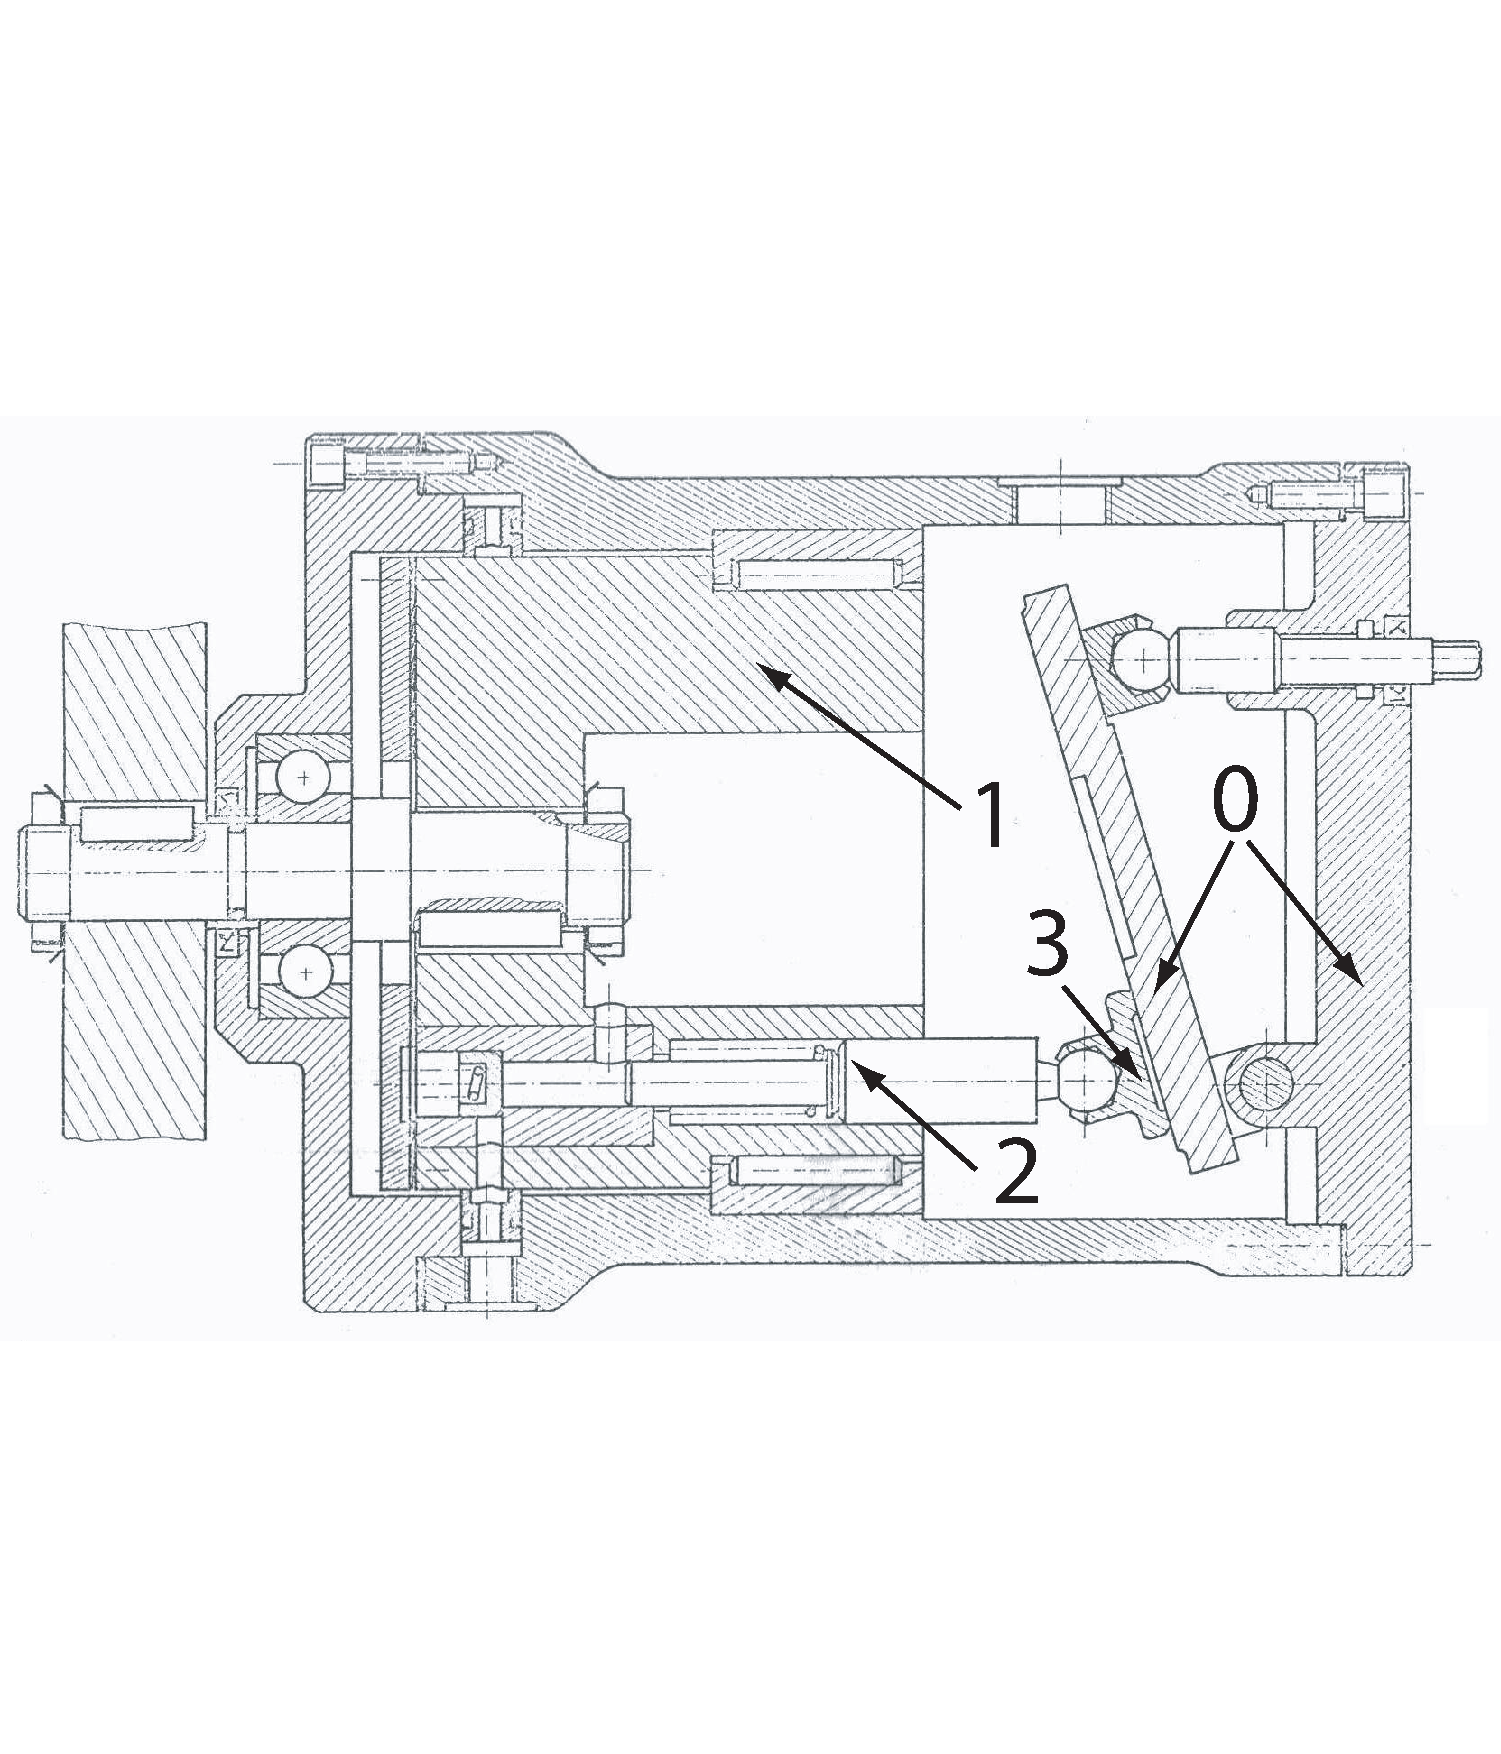
\includegraphics[width=.9\linewidth]{pompe.pdf}
  
  \textit{Schéma technologique d'une pompe à pistons axiaux \label{fig:techno_pompe}}

\end{center}


Les liaisons entre les différentes classes d'équivalence permettent de modéliser le système avec le schéma cinématique ci-après.



\begin{itemize}
\item Les liaisons sont parfaites : sans frottements ni jeux.
\item Le poids et les effets d'inerties sont négligés.
\item On introduit une action de pression s'exerçant sur le piston 2 assimilable à un glisseur d'axe central $\axe{C}{{z_1}}$ et qui a pour résultante en effort : $\vect{F_p}=F_p\vect{z_1}$
\end{itemize}


\begin{center}
 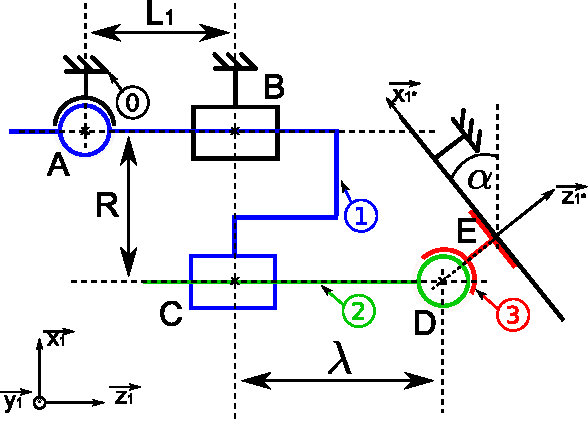
\includegraphics[width=.9\linewidth]{pompe_cine.pdf}
 
 \textit{Schéma cinématique d'une pompe à pistons axiaux \label{fig:cine_pompe}}
\end{center}

\subsection*{Etude préliminaire}
\subparagraph{}\textit{Tracer le graphe de structure du mécanisme.}

\subparagraph{}\textit{En utilisant les formules globales de l'hyperstatisme, déterminer le degré d'hyperstatisme en utilisant la méthode statique puis la méthode cinématique.}


\subsection*{Étude statique}

\subparagraph{}\textit{Isoler successivement les pièces 1, 2 puis 3 et réaliser le PFS en $B$, $C$ et $D$.}

\subparagraph{}\textit{Écrire le système d'équations. Conclure sur le rang du système d'équations et sur l'hyperstatisme du système mécanique.}

\subsection*{Étude cinématique}

\subparagraph{}\textit{Écrire les fermetures de chaînes associées au mécanisme. }
\subparagraph{}\textit{Écrire le système d'équations. Conclure sur le rang du système d'équations et sur l'hyperstatisme du système mécanique.}

\subsection*{Hyperstatisme}
\subparagraph{}\textit{Proposer des conditions géométriques permettant d'assurer l'assemblage du système. }
\subparagraph{}\textit{Proposer une modèle isostatique cinématiquement équivalent. }

\ifprof
\end{multicols}
\else
\end{multicols}
\fi



\subsection*{Objectifs}
\begin{itemize}
\item La résolution statique a pour but de déterminer les actions dans les liaisons mécaniques. Cette résolution pourra alors ensuite permettre un dimensionnement des différentes liaisons.
\item Cette approche permet également de déterminer l'isostaticité ou l'hypertstaticité en vue de d'estimer les conditions éventuelles de montage du mécanisme.
\end{itemize}

\subsection*{Bilan des actions mécanique pour chacune des classes d'équivalence}
\subsubsection*{Bilan des actions mécaniques pour l'ensemble 1}
On choisit d'écrire tous les torseurs des actions mécaniques au point $B$ :
\begin{itemize}
\item \textbf{Action de 0 sur 1 en A :}
%\ifprof
$$
\torseurstat{T}{S_0}{S_{1A}}
=\torseurcol{X_{A01}}{Y_{A01}}{Z_{A01}}{0}{0}{0}{A,R_1}
=\torseurcol{X_{A01}}{Y_{A01}}{Z_{A01}}{L_1\;Y_{A01}}{-L_1\;X_{A01}}{0}{B,R_1}
$$
\item \textbf{Action de 0 sur 1 en B :}
$$
\torseurstat{T}{S_0}{S_{1B}}
=\torseurcol{X_{B01}}{Y_{B01}}{0}{L_{B01}}{M_{B01}}{0}{B,R_1}
$$
\item \textbf{Action de 2 sur 1 en C :}
$$
\torseurstat{T}{S_2}{S_{1}}
=\torseurcol{X_{21}}{Y_{21}}{0}{L_{21}}{M_{21}}{0}{C,R_1}
=\torseurcol{X_{21}}{Y_{21}}{0}{L_{21}}{M_{21}}{-R\;Y_{21}}{B,R_1}
$$

%\else\fi
\end{itemize}

\subsubsection*{Bilan des actions mécaniques pour l'ensemble 2}

On choisit d'écrire tous les torseurs des actions mécaniques au point $C$ :
\begin{itemize}
\item \textbf{Action de 3 sur 2 en D :}\\
%\ifprof
$$
\torseurstat{T}{S_3}{S_2}
=\torseurcol{X_{32}}{Y_{32}}{Z_{32}}{0}{0}{0}{D,R_1}
=\torseurcol{X_{32}}{Y_{32}}{Z_{32}}{-\lambda \;Y_{32}}{\lambda \;X_{32}}{0}{C,R_1}
$$
%\else\fi
\item \textbf{Action de 1 sur 2 en C :}\\
%\ifprof
$$
\torseurstat{T}{S_1}{S_{2}}
=\torseurcol{-X_{21}}{-Y_{21}}{0}{-L_{21}}{-M_{21}}{0}{C,R_1}
$$

%\else\fi
\item \textbf{Action de la pression en C :}\\
%\ifprof
$$
\torseurstat{T}{\text{pression}}{S_{2}}
=\torseurcol{0}{0}{F_p}{0}{0}{0}{C,R_1}
$$
%\else\fi
\end{itemize}

\subsubsection*{Bilan des actions mécaniques pour l'ensemble 3}

On choisit d'écrire tous les torseurs des actions mécaniques au point D :
\begin{itemize}
\item \textbf{Action de 2 sur 3 en D :}\\
%\ifprof
$$
\torseurstat{T}{S_2}{S_3}
=\torseurcol{-X_{32}}{-Y_{32}}{ -Z_{32}}{0}{0}{0}{D,R_1}
$$
%\else\fi
\item \textbf{Action de 0 sur 3 en E :}\\
%\ifprof
$$
\torseurstat{T}{S0}{S3}
=\torseurcol{0}{0}{Z_{03}}{L_{03}}{M_{03}}{0}{C,R_{1*}}
$$
$$
=\torseurcol{0}{0}{Z_{03}}{L_{03}}{M_{03}}{ 0}{D,R_{1*}}$$

$$
=\torseurcol{Z_{03}\sin(\alpha) }{ 0 }{ Z_{03}\cos(\alpha)}{L_{03}\cos(\alpha) }{ M_{03} }{ -L_{03}\sin(\alpha)}{D,R_{1}}
$$
%\else\fi
\end{itemize}






\subsection*{Résolution d'un système linéaire homogène}

En appliquant successivement le principe fondamental de la statique pour chacun des trois ensemble on obtient un système de 18 équations :

\begin{align*}
\begin{array}{c}
(1) \mbox{résultante suivant} \vect{x_1} \\ 
(2) \mbox{résultante suivant} \vect{y_1} \\ 
(3) \mbox{résultante suivant} \vect{z_1} \\ 
(4) \mbox{moment suivant} \axe{B}{{x_1}} \\ 
(5) \mbox{moment suivant} \axe{B}{{y_1}} \\ 
(6) \mbox{moment suivant} \axe{B}{{z_1}} \\ 
(7) \mbox{résultante suivant} \vect{x_1} \\ 
(8) \mbox{résultante suivant} \vect{y_1} \\ 
(9) \mbox{résultante suivant} \vect{z_1} \\ 
(10) \mbox{moment suivant} \axe{C}{{x_1}} \\ 
(11) \mbox{moment suivant} \axe{C}{{y_1}} \\ 
(12) \mbox{moment suivant} \axe{C}{{z_1}} \\ 
(13) \mbox{résultante suivant} \vect{x_1} \\ 
(14) \mbox{résultante suivant} \vect{y_1} \\ 
(15) \mbox{résultante suivant} \vect{z_1} \\ 
(16) \mbox{moment suivant} {D}{\vect{x_1}} \\ 
(17) \mbox{moment suivant} {D}{\vect{y_1}} \\ 
(18) \mbox{moment suivant} {D}{\vect{z_1}} \\ 
\end{array}
%\left\{
\begin{array}{c}
X_{A01}+X_{B01}+X_{C21}=0 \\
Y_{A01}+Y_{B01}+Y_{C21}=0 \\ 
Z_{A01}=0 \\ 
L_1\;Y_{A01}+L_{B01}+L_{C21}=0 \\ 
-L_1\;X_{A01}+M_{B01}+M_{C21}=0 \\  
-R\;Y_{C21} =0\\
X_{D32}-X_{C21}=0 \\ 
Y_{D32}-Y_{C21}=0 \\  
Z_{D32}+F_p=0 \\ 
-\lambda\;Y_{D32}-L_{C21}=0 \\ 
\lambda\;X_{D32}-M_{C21}=0 \\ 
0 =0\\
-X_{D32}+Z_{E03}\sin(\alpha)=0 \\ 
-Y_{D32}=0 \\ 
-Z_{D32}+Z_{E03}\cos(\alpha)=0 \\ 
L_{E03}\cos(\alpha)=0 \\ 
M_{E03}=0\\ 
-M_{E03}\sin(\alpha)=0\\ 
\end{array}%\right.
\end{align*}


\subsection*{Mise en évidence de l'hyperstatisme et de la mobilité}
%\begin
Bilan de l'approche statique
\begin{itemize}
\item On obtient alors un système de \textbf{$E_s=18$ équations statiques}.
\item La modélisation comporte \textbf{$I_s=17$ inconnues statiques}.
\item Certaines de ces équations ne sont pas significatives, elles correspondent aux mobilités cinématiques du mécanisme :
\begin{itemize}
\item Équation (12) \textbf{``$0=0$''} : \textit{mobilité de rotation de piston autour de $\axe{C}{{z_1}}$}.
\item Les équations (6) (8) et (14) sont équivalentes à deux équations libres : \textit{mobilité de rotation du barillet autour de $\axe{B}{{z_1}}$}.
\item Équation (18) liée à (17) : \textit{rotation du poussoir autour de $\axe{E}{{z_{1*}}}$}.		
\end{itemize}
Le système possède alors \textbf{3 mobilités cinématiques ($m_c=3$)}.
		
		Pour résoudre ce système on se retrouve donc avec \textbf{$r_S=15$ équations significatives} (rang du système d'équations statiques $r_s$) pour \textbf{$I_S=17$ inconnues}. Nous avons donc un déficit de \textbf{2 équations} ou encore 2 inconnues statiques de trop pour résoudre le problème. Le système est donc \textbf{hypercontraint}.
		\textbf{On dit que la modélisation du système est hyperstatique d'ordre 2}
\begin{align}\label{hyper_statique}
\boxed{
h=I_s-r_s=I_s-(E_s-m_c)
}
\end{align}
		
\end{itemize}

%\end{bilan} 



%\FloatBarrier
\section*{Étude cinématique}
\subsection*{Objectifs}
\begin{itemize}
\item La résolution cinématique a pour but de déterminer les caractéristiques cinématiques au niveau de toutes les liaisons de la chaîne.
\item Cette approche permet également de déterminer l'isostaticité ou l'hypertstaticité en vue de déterminer les conditions éventuelles de montage du mécanisme.
\item Elle permet enfin de déterminer la loi entrée-sortie cinématique du mécanisme.
\end{itemize}
\subsection*{Démarche}
Le graphe de liaison donné ci-après montre que le mécanisme possède deux chaînes fermées :
\begin{itemize}
\item Chaîne 1 : $\left\{0-3-2-1-0\right\}$.
\item Chaîne 2 : $\left\{0-1-0\right\}$.
\end{itemize}
L'approche cinématique consiste à écrire pour chaque chaine la fermeture cinématique à l'aide des torseurs.




\begin{center}
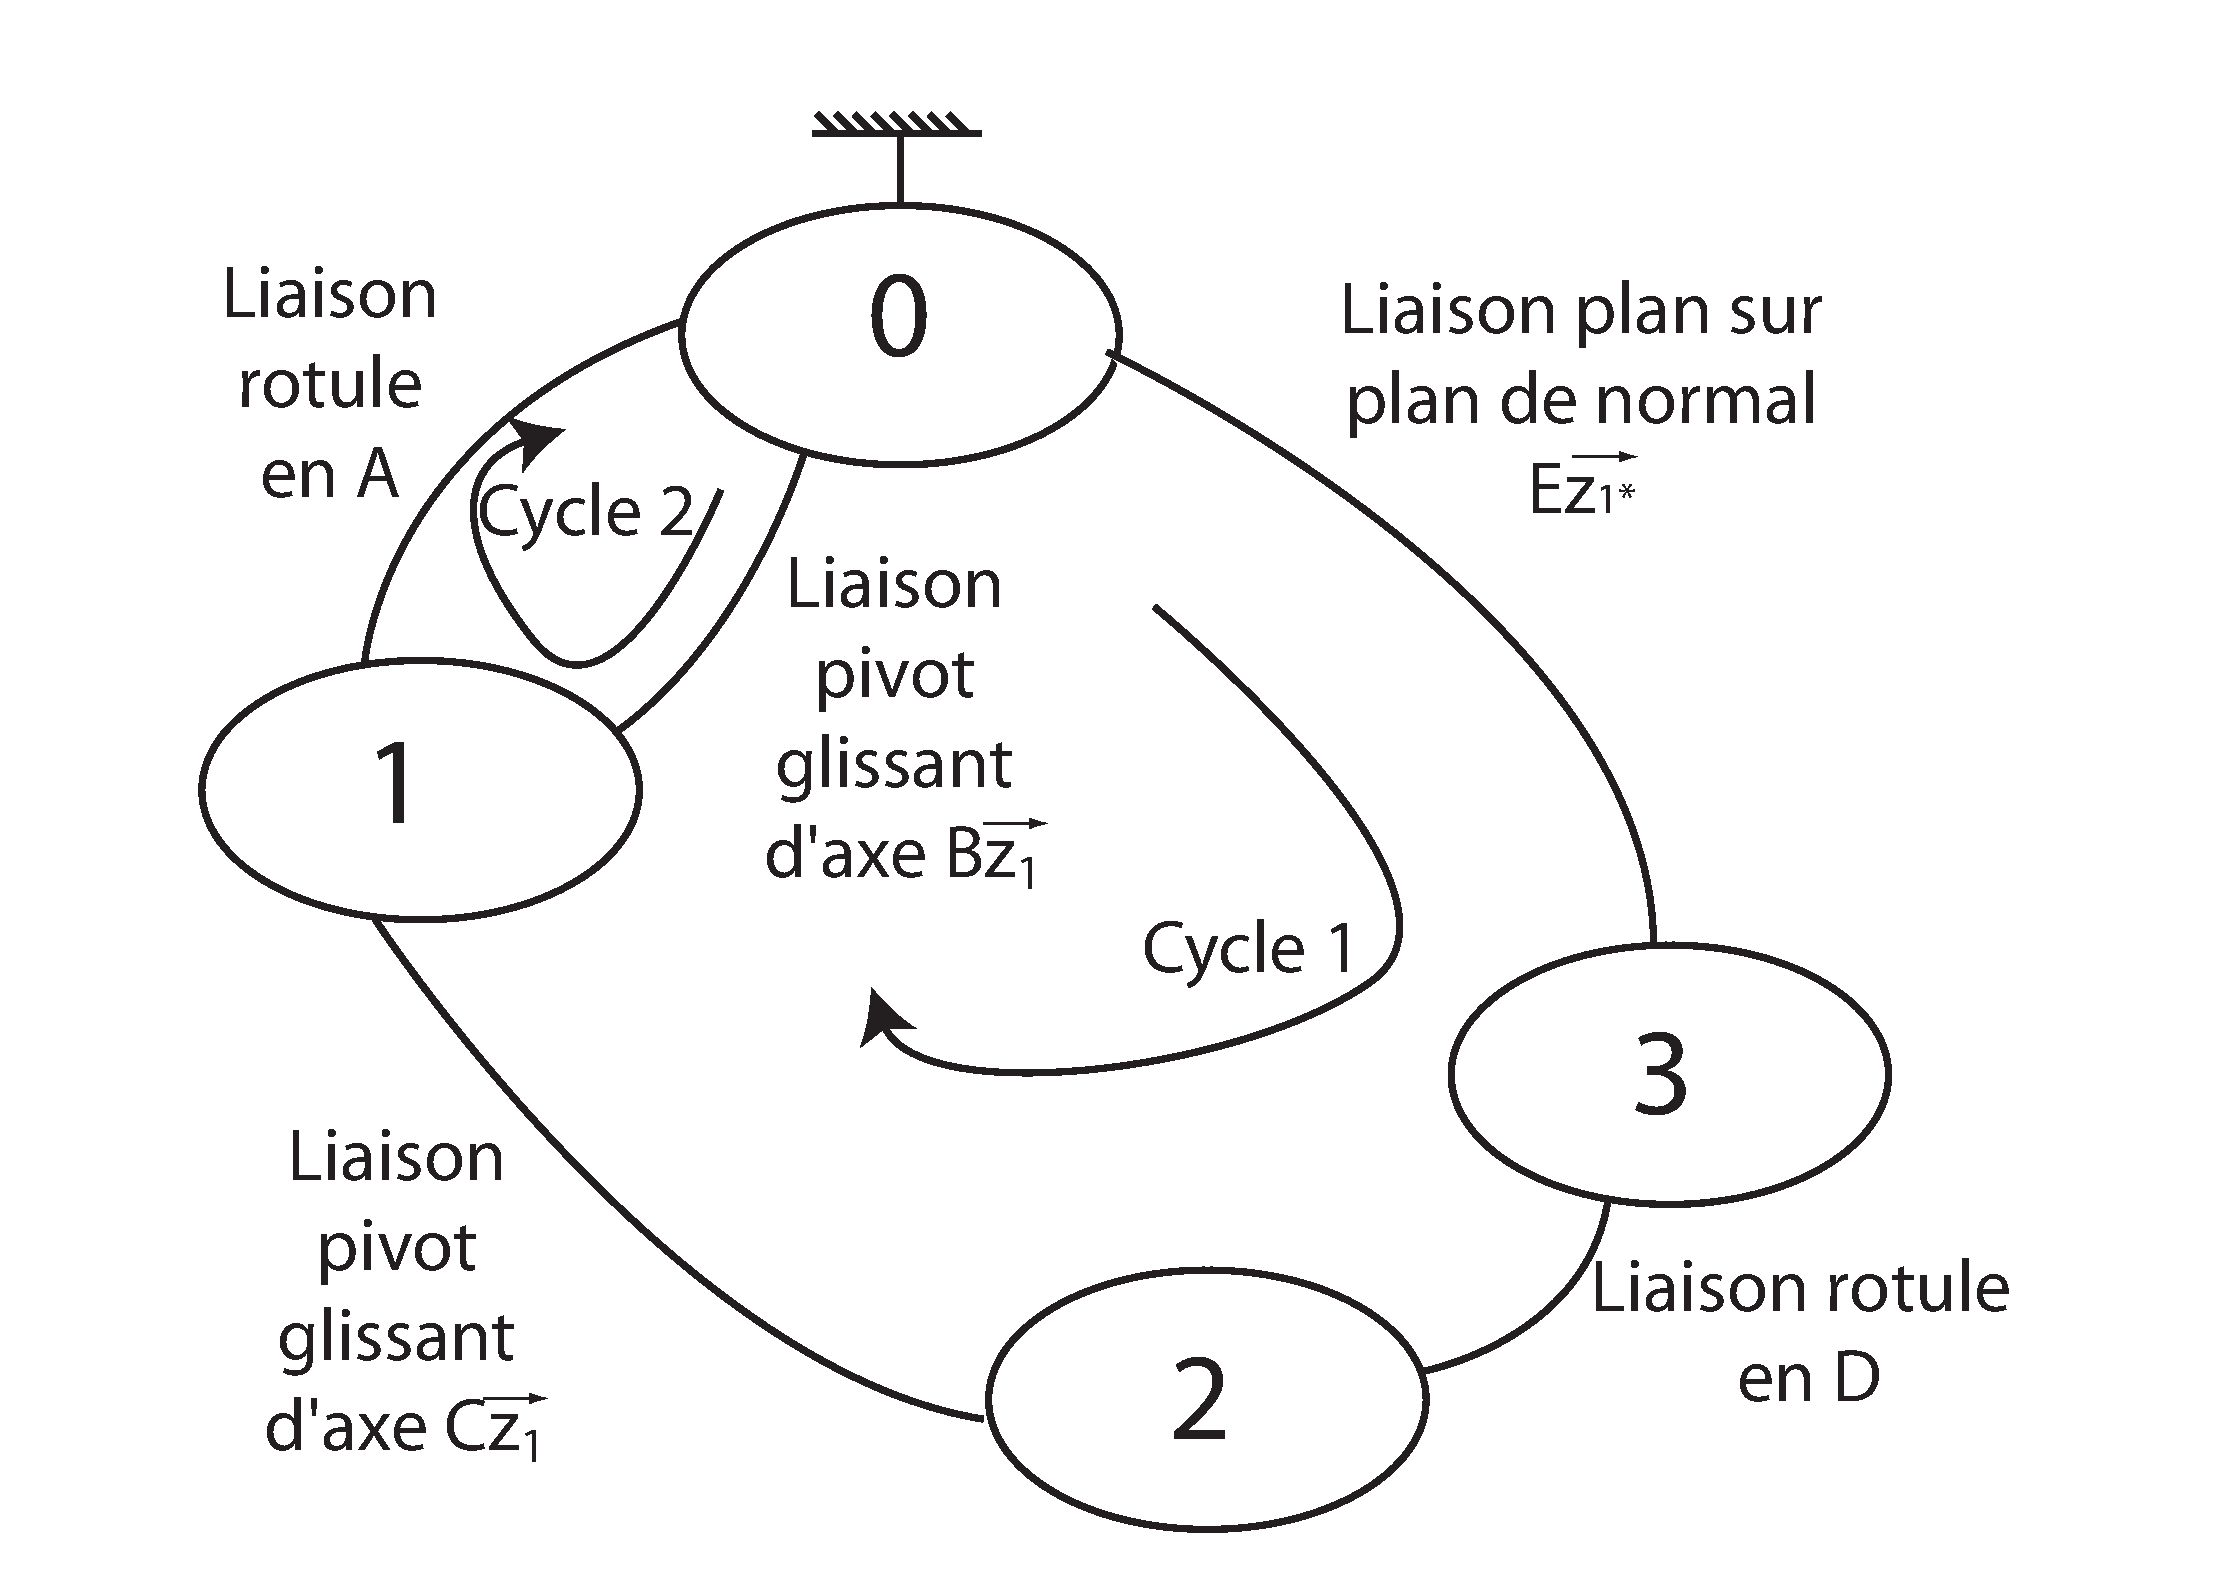
\includegraphics[width=\linewidth]{graph_structure_pompe2.pdf}

\textit{Graphe de structure de la pompe \label{fig:graphe_structure_pompe2}}
\end{center}


%\FloatBarrier
\subsection*{Fermeture de chaine cinématique}
\subsubsection*{Chaine cinématique 1}

La fermeture cinématique s'écrit :
$$
\torseurcin{V}{3}{0} = \torseurcin{V}{3}{2}
+\torseurcin{V}{2}{1}
+\torseurcin{V}{1}{0}
$$
		On détermine alors successivement les différents torseurs cinématiques que l'on exprimera tous en $C$:

		\begin{itemize}
\item \textbf{$\torseurcin{V}{3}{0}$}:\\
$$
\torseurcin{V}{3}{0}	
=	\torseurcol{0}{0}{r_{30}}{u_{30}}{v_{30}}{0}{E,R_{1*}}
$$
$$
=	\torseurcol{0}{0}{{r}_{30}}{u_{30}}{v_{30}}{0}{D,R_{1*}}\\
=	\torseurcol{0}{r_{30}\;\sin(\alpha)}{r_{30}\;\cos(\alpha)}{u_{30}\;\cos(\alpha)}{v_{30}}{-u_{30}\;\sin(\alpha)}{D,R_{1}}
$$
$$
=\torseurcol{0}{r_{30}\;\sin(\alpha)}{r_{30}\;\cos(\alpha)}{u_{30}\;\cos(\alpha)-\lambda\;r_{30}\;\sin(\alpha)}{v_{30}}{-u_{30}\;\sin(\alpha)}{C,R_{1}}
$$
\item \textbf{$\torseurcin{V}{3}{2}$}:\\
$$
\torseurcin{V}{3}{2}	
=	\torseurcol{p_{32}}{q_{32}}{r_{32}}{0}{0}{0}{D,R_{1}}
=	\torseurcol{p_{32}}{q_{32}}{r_{32}}{-\lambda\;q_{32}}{\lambda\;p_{32}}{0}{C,R_{1}}
$$
\item \textbf{$\torseurcin{V}{2}{1}$}:\\
$$
\torseurcin{V}{2}{1}	
=	\torseurcol{0}{0}{r_{21}}{0}{0}{w_{21}}{C,R_{1}}
$$
\item \textbf{$\torseurcin{V}{1}{0}$}:\\
$$
\torseurcin{V}{1}{0}	
=	\torseurcol{0}{0}{r_{B10}}{0}{0}{0}{B,R_{1}}
=	\torseurcol{0}{0}{r_{B10}}{0}{-R\;r_{B10}}{0}{C,R_{1}}
$$
\end{itemize}
		


\subsubsection*{Chaine cinématique 2}
La fermeture cinématique s'écrit :

		$$\torseurcin{V}{1_A}{0}=	\torseurcin{V}{1_B}{0}$$
		
		On détermine alors successivement les différents torseurs cinématiques que l'on exprimera tous en $A$:

		\begin{itemize}
\item \textbf{$\torseurcin{V}{1_A}{0}$}:\\
$$
\torseurcin{V}{1_A}{0}	
=	\torseurcol{p_{A10}}{q_{A10}}{r_{A10}}{0}{0}{0}{A,R_{1}}
$$
\item \textbf{$\torseurcin{V}{1_B}{0}$}:\\
$$
\torseurcin{V}{1_B}{0}
=	\torseurcol{0}{0}{r_{B10}}{0}{0}{w_{B10}}{A,R_{1}}
$$

\end{itemize}



\subsection*{Résolution}
On écrit alors la fermeture cinématique pour chaque fermeture cinématique. Cela donnera 12 équation pour 13 inconnues avec les deux fermetures de chaines :

\begin{align*}
\torseur{\mathcal{V}^{A}_{(1/0)}}-\torseur{\mathcal{V}^{B}_{(1/0)}}=\left\{0\right\}\\
\\
\torseurcin{V}{3}{2}+	\torseurcin{V}{2}{1}	
+	\torseurcin{V}{1}{0}-\torseurcin{V}{3}{0}	=\left\{0\right\}
\end{align*}
\begin{align*}
\begin{array}{c}
(1)\\
(2)\\
(3)\\
(4)\\
(5)\\
(6)\\
(7)\\
(8)\\
(9)\\
(10)\\
(11)\\
(12)\\
\end{array}
\left(
\begin{array}{ccccccccccccc}
1 & 0 & 0 & 0 & 0 & 0 & 0 & 0 & 0 & 0 & 0 & 0 & 0 \\
0 & 1 & 0 & 0 & 0 & 0 & 0 & 0 & 0 & 0 & 0 & 0 & 0 \\ 
0 & 0 & 1 & -1 & 0 & 0 & 0 & 0 & 0 & 0 & 0 & 0 & 0 \\ 
0 & 0 & 0 & 0 & 0 & 0 & 0 & 0 & 0 & 0 & 0 & 0 & 0 \\ 
0 & 0 & 0 & 0 & 0 & 0 & 0 & 0 & 0 & 0 & 0 & 0 & 0 \\ 
0 & 0 & 0 & 0 & 1 & 0 & 0 & 0 & 0 & 0 & 0 & 0 & 0 \\  
0 & 0 & 0 & 0 & 0 & 0 & 0 & 0 & 1 & 0 & 0 & 0 & 0 \\ 
0 & 0 & 0 & 0 & 0 & 0 & 0 & -\sin(\alpha) & 0 & 1 & 0 & 0 & 0 \\
0 & 0 & 0 & 1 & 0 & 0 & 0 & -\cos(\alpha) & 0 & 0 & 1 & 1 & 0 \\
0 & 0 & 0 & 0 & 0 & -\cos(\alpha) & 0 & \lambda \;\sin(\alpha) & 0 & -\lambda & 0 & 0 & 0 \\ 
0 & 0 & 0 & -R & 0 & 0 & -1 & 0 & \lambda & 0 & 0 & 0 & 0 \\
0 & 0 & 0 & 0 & 0 & \sin(\alpha) & 0 & 0 & 0 & 0 & 0 & 0 & 1 \\ 
\end{array} 
\right)
\cdot 
\left(
\begin{array}{c}
p_{A10}\\
q_{A10}\\
r_{A10}\\
r_{B10}\\
w_{B10}\\
u_{30}\\
v_{30}\\
r_{30}\\
p_{32}\\
q_{32}\\
r_{32}\\
r_{21}\\
w_{21}
\end{array}
\right)
=
\left(
\begin{array}{c}
0\\
0\\
0\\
0\\
0\\
0\\
0\\
0\\
0\\
0\\
0\\
0\\
\end{array}
\right)
\end{align*}
			

	
\subsection*{Mise en évidence de l'hyperstatisme et de la mobilité}
\subsubsection*{Approche cinématique}
\begin{itemize}
\item Avec deux cycles fermés, on obtient alors un système de $E_c=12$ équations.
\item La modélisation comporte $I_c=13$ inconnues cinématiques.
\item Le rang du système vaut $r_c=10$ car deux équations ((4) et (5)) donnent \textbf{``$0=0$''} et ne sont donc pas significatives.
\item Le nombre d'équations non-significatives correspond directement à l'\textbf{hyperstaticité} (ici $h=2$) 
\item La mobilité cinématique se définit comme la différence entre le nombre d'inconnues cinématiques ($I_c$) et le nombre d'équations significatives ($r_c$) : \textbf{ici $mc=3$}

\begin{align}\label{hyper_cine}
\boxed{
m_c=I_c-r_c=I_c-(E_c-h).
}
\end{align}
		

\end{itemize}



			
%\end{multicols}


\section*{Hyperstatisme}



	\subsection*{Degrés de mobilité}
	%-----------------------------------------------------------

	
		
		\begin{definition}[Mobilité cinématique]
		On appelle $m_c=m_u+m_i$ le \textbf{degrés de mobilité cinématique} d'une liaison ou d'un mécanisme, avec :
			\begin{itemize}
				\item $m_u$ : le nombre de mobilités dites \textbf{utile},
				\item $m_i$ : le nombre de mobilités dites \textbf{interne}.
			\end{itemize}
		\end{definition}

		Pour une liaison seule :
		\begin{itemize}
			\item $m_c=0$ : liaison complète ou rigide,
			\item $m_c>0$ : liaison mobile à $m_c$ degrés de liberté.
		\end{itemize}

		\begin{rem}
			\item Dans un mécanisme, une mobilité utile est une mobilité \textbf{recherchée dans la fonction du mécanisme}.
				On différenciera \textbf{seulement} les mobilités utiles \textbf{indépendantes}.
				Si une relation existe, par exemple, entre un mouvement d'entrée et un mouvement de sortie, alors cela sera considéré comme une seule mobilité.
			\item Les mobilités internes sont des mobilités indépendantes résiduelles à l'intérieur du mécanisme.
		\end{rem}



